\section{Ejercicio 8}


\subsection{Desarrollo}
Similar  a lo visto en el ejercicio 4, tendremos que programar la estructura de un scheduler de Round-Robin. La diferencia es que en este caso en vez de tener una cola única 
que vaya guardando todos los procesos, cada core tendrá su propia cola de procesos. Para resolver esto utilizaremos una estructura para representar el core que nos dará la 
siguiente información: un entero pidActual, un entero cpu$\_$quantum, un entero quantum$\_$restantes, su cola de pids enEspera, un vector pid$\_$bloqueados que indica cuales están en ese estado.

Después tenemos la cantidad de cores y el quantum de los mismos. Por último necesitamos agrupar las estructuras core que tenemos. Para esto usamos simplemente un vector 
(nucleos).

La función load lo que hace es buscar cual de los cores tiene menor cantidad de procesos(suma los bloqueados, los de enEspera y el de pidActual, si no es IDLE). Una vez 
encontrado, lo encola en el enEspera del core.

unblock lo que hace es buscar cual es el core donde se encuentra el pid que se desea bloquear, una vez encontrado lo quita de pid$\_$bloqueados y lo pone en enEspera.

Por último tenemos la función tick. El código es equivalente al del ejercicio 4.


\subsection{Experimentación}
Según lo pedido debemos mencionar un caso donde la migración de núcleos sea beneficiosa y otro donde no. Para lo primero, usaremos dos core y cuatro tareas que irán apareciendo
en este orden: la más costosa,  la menos costosa, la segunda más costosa y la segunda menos costosa. Usaremos, en los dos cores, un quantum de 5(para todos) y nos queda lo siguiente:

TaskCPU 100   	//Costosa

@1:

TaskCPU 10 	//Poco Costosa

@2:

TaskCPU 80 	//Costosa

@3:

TaskCPU 20 	//Poco Costosa

\begin{figure}[H]
  \centering
    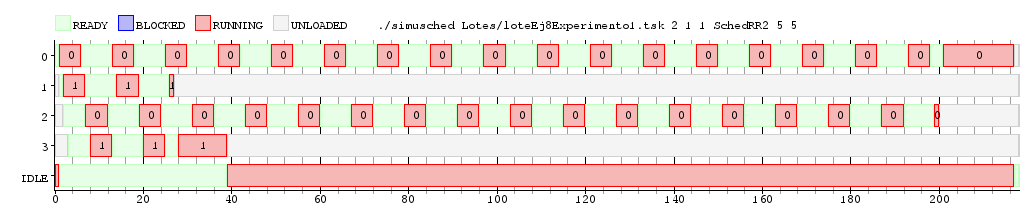
\includegraphics[width=1.1\textwidth]{imagenes/Ej8Experimento1.png}
  \caption{loteEj8Experimento1.tsk con RR}
\end{figure}

\begin{tabular}{l | r | r | r }
  Proceso & Latencia & Waiting time & Tiempo total\\
  \hline
  Tarea 0 & 1 & 30 & 131 \\
  Tarea 1 & 1 & 15 & 26 \\
  Tarea 2 & 5 & 28 &  109\\
  Tarea 3 & 5 & 30 & 51\\
  Promedio & 3 & 25.75 & 79.25\\
\end{tabular}

\begin{figure}[H]
  \centering
    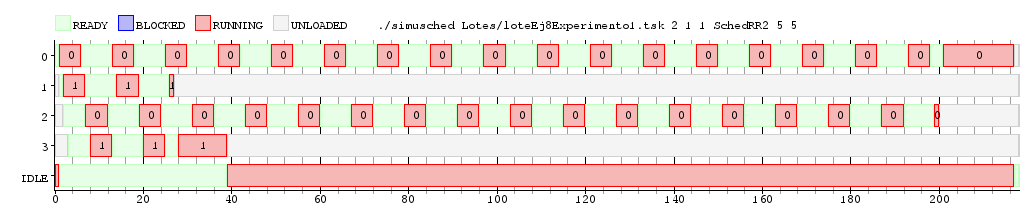
\includegraphics[width=1.1\textwidth]{imagenes/Ej8Experimento2.png}
  \caption{loteEj8Experimento1.tsk con RR2}
\end{figure}

\begin{tabular}{l | r | r | r }
  Proceso & Latencia & Waiting time & Tiempo total\\
  \hline
  Tarea 0 & 1 & 116 &  216\\
  Tarea 1 & 1 & 15 &  22\\
  Tarea 2 & 5 & 117 & 198 \\
  Tarea 3 & 5 & 15 & 36\\
  Promedio & 3 & 65.75 & 118 \\
\end{tabular}

Podemos ver que la corrida con el RR2 tarda más en terminar las tareas más costosa respecto a lo que tarda RR(todas excepto la Tarea 1). Esto se debe a que solo son atendidas 
por un cpu mientras el otro ejecuta tareas de bajo costo y, por lo tanto, termina antes y se queda inactivo mientras el otro sigue trabajando. Mientras tanto el que posee 
migración de núcleos. 
Las más costosas tienen un peor waiting time. También se ve que tiempo final promedio y el waiting time promedio es mayor en la que no tiene migración de núcleos. Por
lo tanto para este lote es mejor el scheduler con migración de núcleos. 

Para el caso donde es peor utilizaremos el siguiente lote de tareas:

TaskCPU 100

@6:

TaskCPU 30

@12:

TaskCPU 30

El cambio es que las ejecuciones tendrán un costo de migración de núcleos de 10(en los anteriores experimentos era de 1).

\begin{figure}[H]
  \centering
    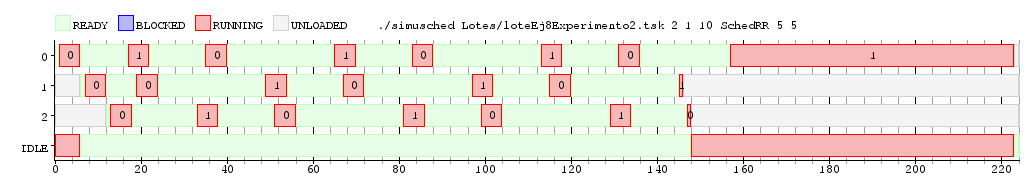
\includegraphics[width=1.1\textwidth]{imagenes/Ej8Experimento3.png}
  \caption{loteEj8Experimento2.tsk con RR}
\end{figure}

\begin{tabular}{l | r | r | r }
  Proceso & Latencia & Waiting time & Tiempo total\\
  \hline
  Tarea 0 & 1 & 122 &  223\\
  Tarea 1 & 1 & 109 &  140\\
  Tarea 2 & 5 & 105 & 132 \\
  Promedio & 2.33 & 112 & 165 \\
\end{tabular}

\begin{figure}[H]
  \centering
    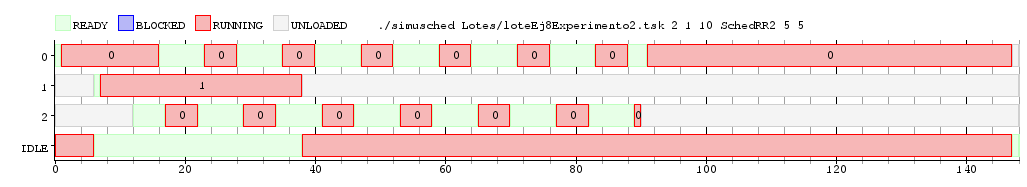
\includegraphics[width=1.1\textwidth]{imagenes/Ej8Experimento4.png}
  \caption{loteEj8Experimento2.tsk con RR2}
\end{figure}

\begin{tabular}{l | r | r | r }
  Proceso & Latencia & Waiting time & Tiempo total\\
  \hline
  Tarea 0 & 1 & 46 &  147\\
  Tarea 1 & 1 & 1 &  32\\
  Tarea 2 & 5 & 47 & 78 \\
  Promedio & 2.33 & 31.33 & 85.66 \\
\end{tabular}

Podemos ver que, en este caso, el waiting time promedio y el tiempo total promedio son mejores en el que no tiene migración de núcleos. Esto es debido a que el scheduler RR2
no paga el costo de migración porque cada tarea se ejecuta siempre en el mismo núcleo, mientras que RR cada vez que desaloja una tarea tarda más tiempo si la próxima no se estuvo
ejecutando en el mismo core. El lote esta pensado para que esto suceda.
